\chapter{Counting}\label{chapter:combinatorial-methods}

\section{Hume's Principle}

Combinatorics, or discrete mathematics,
is the mathematics of finite structures.
A central theme in combinatorics is counting,
establishing a closed form for the number of objects of a certain kind.
Such counting methods can sometimes be used to obtain results in number theory.
For instance, we will use a counting argument to show that the product
\begin{equation*}
  n(n-1)\cdots(n-k+1)
\end{equation*}
of any $k$ consecutive natural numbers is always divisible by $k!$.

What do mathematicians mean by counting? How do we establish that a certain set of objects contain a certain number of objects? Or, more generally, how do we establish that two sets of objects have the same number of objects?

These questions take us back to the 18\supth{}-century Scottish philosopher David Hume. He sheds light on this very question in his \textsc{Treatise of Human Nature},
a philosphical work in which he set out to found a general ``science of man'' by applying empirical methods to understanding, the passions, and morals \cite[Part III, Book I]{hume1978}.
In discussing the idea of number, he observes that equality of numbers can be determined whenever there is a one-to-one correspondence between their constituents:
\begin{quote}
  {\itshape We are possest of a precise standard, by which we can judge
    of the equality and proportion of numbers; and according as they correspond
    or not to that standard, we determine their relations, without any
    possibility of error. When two numbers are so combin'd, as that the one has
    always an unite answering to every unite of the other, we pronounce them
    equal; and 'tis for want of such a standard of equality in extension, that
    geometry can scarce be esteem'd a perfect and infallible science.}
\end{quote}
We note here that Hume relies on the Euclidean conception of number,
where a number is a multitude of units:
the number $n$ is the collection of $n$ units.
By contrast,
in modern mathematics we treat the natural numbers as an inductively generated set.
To recover Hume's insight in our setting,
we introduce the notion of a standard $n$-element set,
which is to be a fixed set with exactly $n$ elements playing the role of Euclid's collection of $n$ units.

\begin{definition}
  The \define{standard finite set} $[n]$ with $n$ elements is defined by
  \begin{equation*}
    [n]:=\{0,\ldots,n-1\}=\{x\in\mathbb{N}\mid x<n\}.
  \end{equation*}
\end{definition}

The standard $0$-element set $[0]$ is the empty set,
since there are no natural numbers strictly smaller than $0$.
The standard $1$-element set is the set $\{0\}$,
since $0$ is the only element strictly smaller than $1$.
The standard $2$-element set is the set $\{0,1\}$,
since the only two elements strictly smaller than $2$ are $0$ and $1$,
and so forth.

\begin{figure}[t]
  \centering
  \begin{tikzpicture}[
    alt={Two sets with three elements each, and arrows between their elements so as to indicate a bijective correspondence. The elements of the first set A are labeled a_1, a_2, a_3, and the elements of the second set B are labeled b_1, b_2, b_3. The bijection sends a_1 to b_2, a_2 to b_3, and a_3 to b_1.},
    element/.style={circle, draw, thick, minimum size=6mm, inner sep=0pt},
    set/.style={ellipse, draw=CornflowerBlue, thick, minimum height=35mm, minimum width=20mm},
    underpass/.style={draw=white, line width=3pt, bend left=10, shorten >=2mm, shorten <=2mm},
    mapsto/.style={
      |->,
      thick,
      bend left=10,
      shorten >=2mm,
      shorten <=2mm
    },
    ]
    
    % Left set (domain)
    \node[set,label=left:$A$] (A) at (0,0) {};
    \node[element] (a1) at ($(A.center)+(0,1.2)$) {$a_1$};
    \node[element] (a2) at ($(A.center)+(0,0)$) {$a_2$};
    \node[element] (a3) at ($(A.center)+(0,-1.2)$) {$a_3$};
    
    % Right set (codomain)
    \node[set,label=right:$B$] (B) at (5,0) {};
    \node[element] (b1) at ($(B.center)+(0,1.2)$) {$b_1$};
    \node[element] (b2) at ($(B.center)+(0,0)$) {$b_2$};
    \node[element] (b3) at ($(B.center)+(0,-1.2)$) {$b_3$};
    
    % Bijection arrows
    \draw[underpass] (a1) to (b2);
    \draw[mapsto] (a1) to (b2);
    \draw[underpass] (a2) to (b3);
    \draw[mapsto] (a2) to (b3);
    \draw[underpass] (a3) to (b1);
    \draw[mapsto] (a3) to (b1);
    
  \end{tikzpicture}
  \caption[A bijection]{A bijection between two $3$-element sets.}
  \label{figure:bijection}
\end{figure}

Suppose now that we are given an arbitrary set $A$,
and we wish to count its elements.
What does it mean when we say that the set $A$ has $n$ elements?
It means that we can, at least in principle,
label each element of $A$ with a number $0\leq i<n$ in such a way that every element of $A$ is labeled by \emph{exactly one} number $0\leq i<n$.
By making sure that every element of $A$ is labeled \emph{at least once} we make sure that every element of $A$ is accounted for,
and by making sure that every element of $A$ is labeled \emph{at most once} we make sure to not overshoot the count.

Thus,
in order to show that the set $A$ has $n$ elements,
we have to create what is called a \define{bijective correspondence} between the elements of the standard finite set $[n]$ and the set $A$.

\begin{definition}
  A function $f:X\to Y$ is said to be a \define{bijection} if for every $y\in Y$ there is exactly one element $x\in X$ such that $f(x)=y$.
  The set of bijections from $X$ to $Y$ is denoted by
  \begin{equation*}
    X\cong Y.
  \end{equation*}
  Furthermore, we say that $X$ \define{is an $n$-element set} if there exists a bijection $[n]\cong X$.
\end{definition}

\begin{figure}[t]
  \centering
  \begin{minipage}[t]{.45\textwidth}
    \centering
    \begin{tikzpicture}[
      alt={A 3-element set A and a 2-element set B, with arrows between the elements of A and the elements of B so as to indicate a function from A to B. This function sends a_1 to b_1, a_2 to b_2, and a_3 to b_1.},
      scale=.9,
      element/.style={circle, draw, thick, minimum size=6mm, inner sep=0pt},
      set/.style={ellipse, draw=CornflowerBlue, thick, minimum height=35mm, minimum width=20mm},
      mapsto/.style={|->, thick, bend left=10, shorten >=2mm, shorten <=2mm},
      underpass/.style={draw=white, line width=3pt, bend left=10, shorten >=2mm, shorten <=2mm}
      ]

      \path[use as bounding box] (-1.2,-2) rectangle (4.2,2);
      
      \node[set,label=left:$A$] (A) at (0,0) {};
      \node[element] (a1) at ($(A.center)+(0,1.2)$) {$a_1$};
      \node[element] (a2) at ($(A.center)+(0,0)$) {$a_2$};
      \node[element] (a3) at ($(A.center)+(0,-1.2)$) {$a_3$};
      
      \node[set,label=right:$B$] (B) at (3,0) {};
      \node[element] (b1) at ($(B.center)+(0,0.6)$) {$b_1$};
      \node[element] (b2) at ($(B.center)+(0,-0.6)$) {$b_2$};
      
      \draw[underpass] (a1) to (b1);
      \draw[mapsto] (a1) to (b1);
      \draw[underpass] (a2) to (b2);
      \draw[mapsto] (a2) to (b2);
      \draw[underpass] (a3) to (b1);
      \draw[mapsto] (a3) to (b1);
      
    \end{tikzpicture}%
    \captionof{figure}[Not a bijection]{This function is not a bijection since the distinct elements $a_1$ and $a_3$ are both sent to $b_1$.}
    \label{figure:not-bijection-1}%
  \end{minipage}%
  %
  \tagpdfsetup{float/split}%
  %
  \hspace{.1\textwidth}%
  \begin{minipage}[t]{.45\textwidth}
    \centering
    \begin{tikzpicture}[
      alt={A 3-element set A and a 4-element set B, with arrows between the elements of A and the elements of B so as to indicate a function from A to B. This function sends a_1 to b_2, a_2 to b_3, and a_3 to b_1.},
      scale=.9,
      element/.style={circle, draw, thick, minimum size=6mm, inner sep=0pt},
      set/.style={ellipse, draw=CornflowerBlue, thick, minimum height=35mm, minimum width=20mm},
      mapsto/.style={|->, thick, bend left=10, shorten >=2mm, shorten <=2mm},
      underpass/.style={draw=white, line width=3pt, bend left=10, shorten >=2mm, shorten <=2mm}
      ]

      \path[use as bounding box] (-1.2,-2) rectangle (4.2,2);
      
      \node[set,label=left:$A$] (A) at (0,0) {};
      \node[element] (a1) at ($(A.center)+(0,1.2)$) {$a_1$};
      \node[element] (a2) at ($(A.center)+(0,0)$) {$a_2$};
      \node[element] (a3) at ($(A.center)+(0,-1.2)$) {$a_3$};
      
      \node[set,label=right:$B$] (B) at (3,0) {};
      \node[element] (b1) at ($(B.center)+(0,1.2)$) {$b_1$};
      \node[element] (b2) at ($(B.center)+(0,0.4)$) {$b_2$};
      \node[element] (b3) at ($(B.center)+(0,-0.4)$) {$b_3$};
      \node[element] (b4) at ($(B.center)+(0,-1.2)$) {$b_4$};
      
      \draw[underpass] (a1) to (b2);
      \draw[mapsto] (a1) to (b2);
      \draw[underpass] (a2) to (b3);
      \draw[mapsto] (a2) to (b3);
      \draw[underpass,bend left=20] (a3) to (b1);
      \draw[mapsto,bend left=20] (a3) to (b1);
      
    \end{tikzpicture}%
    \captionof{figure}[Not a bijection]{This function is not a bijection since $b_4$ is not the value of any element in $A$.}%
    \label{figure:not-bijection-2}%
  \end{minipage}
\end{figure}
In \zcref{figure:bijection} we displayed an example of a bijection between two $3$-element sets.
Note that such a bijection would not exist between $A$ and $B$ if the number of elements in $B$ was different from three.
If $B$ had fewer than $3$ elements, as shown in \zcref{figure:not-bijection-1},
then any function $f:A\to B$ would necessarily repeat a value,
while if $B$ had more than $3$ elements,
as shown in \zcref{figure:not-bijection-2},
then no function $f:A\to B$ could have all the elements of $B$ in its range.

This is precisely the reason why we are interested in bijections:
If there is a bijection between $A$ and $B$,
then they must have the same number of elements.
The principle that any two finite sets have the same number of elements if and only if there is a bijection between them is \define{Hume's Principle}.

In order to prove Hume's principle more formally,
we need two lemmas.
The first is an abstract lemma that asserts that two bijections $f:A\cong B$ and $g:B\cong C$ can be composed into a bijection $g\circ f:A\cong C$.
The second is a self-evident looking lemma that establishes that if $A$ is an $(n+1)$-element set and $a\in A$,
then the set $A\setminus\{a\}$ consisting of all elements of $A$ except $a$ is an $n$-element set.
Indeed, such a lemma also requires proof.

Before we state the composability of bijections,
a few comments about how to prove that a function is a bijection and how to use the assumption that a function is a bijection are in order.

\emph{Proving that $f:X\to Y$ is a bijection}.
The condition that a function $f:X\to Y$ is a bijection states that for every element $y\in Y$ there is a unique element $x\in X$ such that $f(x)=y$.
Such unique existence properties have two parts:
first we have to show that there indeed exists at least one such $x$,
and second we have to show that it is unique.
For the second part,
we assume that if both $x$ satisfies $f(x)=y$ and $x'$ satisfies $f(x')=y$,
then we must have $x=x'$.

\emph{Using the condition that $f:X\to Y$ is a bijection}.
If we assume that $f:X\to Y$ is a bijection,
then we have for every $y\in Y$ access to an element $x\in X$ such that $f(x)=y$.
Furthermore,
for every $x'\in X$ such that $f(x')=y$ we know that the equality $x=x'$ must hold,
which we may use if it helps us in our proof.

\begin{figure}[t]
  \centering
  \begin{tikzpicture}[
    alt={Three sets A, B, and C, with bijections between A and B and between B and C. The bijection between A and B sends a sub 1 to b sub 2, a sub 2 to b sub 3, and a sub 3 to b sub 1. The bijection between B and C sends b sub 1 to c sub 2, b sub 2 to c sub 1, and b sub 3 to c sub 3. The composite bijection therefore sends a sub 1 via b sub 2 to c sub 1, a sub 2 via b sub 3 to c sub 3, and a sub 3 via b sub 1 to c sub 2.
    },
    element/.style={circle, draw, thick, minimum size=6mm, inner sep=0pt},
    set/.style={ellipse, draw=CornflowerBlue, thick, minimum height=35mm, minimum width=20mm},
    mapsto/.style={|->, thick, bend left=10, shorten >=2mm, shorten <=2mm},
    underpass/.style={draw=white, line width=3pt, bend left=10, shorten >=2mm, shorten <=2mm}
    ]
    
    \node[set,label=left:$A$] (A) at (0,0) {};
    \node[element] (a1) at ($(A.center)+(0,1.2)$) {$a_1$};
    \node[element] (a2) at ($(A.center)+(0,0)$) {$a_2$};
    \node[element] (a3) at ($(A.center)+(0,-1.2)$) {$a_3$};
    
    \node[set,label=right:$B$] (B) at (4,0) {};
    \node[element] (b1) at ($(B.center)+(0,1.2)$) {$b_1$};
    \node[element] (b2) at ($(B.center)+(0,0)$) {$b_2$};
    \node[element] (b3) at ($(B.center)+(0,-1.2)$) {$b_3$};

    \node[set,label=right:$C$] (C) at (8,0) {};
    \node[element] (c1) at ($(C.center)+(0,1.2)$) {$c_1$};
    \node[element] (c2) at ($(C.center)+(0,0)$) {$c_2$};
    \node[element] (c3) at ($(C.center)+(0,-1.2)$) {$c_3$};

    % Bijection arrows
    \draw[underpass] (a1) to (b2);
    \draw[mapsto] (a1) to (b2);
    \draw[underpass] (a2) to (b3);
    \draw[mapsto] (a2) to (b3);
    \draw[underpass] (a3) to (b1);
    \draw[mapsto] (a3) to (b1);
    \draw[underpass] (b1) to (c2);
    \draw[mapsto] (b1) to (c2);
    \draw[underpass] (b2) to (c1);
    \draw[mapsto] (b2) to (c1);
    \draw[underpass] (b3) to (c3);
    \draw[mapsto] (b3) to (c3);
    
  \end{tikzpicture}
  \caption[Composition of bijections]{Composition of bijections between 3-element sets.}
  \label{figure:composition-of-bijections}
\end{figure}

\begin{lemma}
  Consider two bijections $f:A\cong B$ and $g:B\cong C$. Then the \define{composite} function $g\circ f$ defined by $a\mapsto g(f(a))$, as illustrated in \zcref{figure:composition-of-bijections}, is also a bijection.
\end{lemma}

\begin{proof}
  We have to show that for every element $z\in C$ there is exactly one element $x\in A$ such that $g(f(x))=z$.

  Since $g$ is assumed to be a bijection, there is exactly one element $y\in B$ such that $g(y)=z$. Furthermore, since $f$ is assumed to be a bijection there is exactly one element $x\in A$ such that $f(x)=y$. For such $x$, we have
  \begin{equation*}
    g(f(x))=g(y)=z.
  \end{equation*}
  Thus we have shown that there is at least one such element $x$.

  To see that there is at most one, let $x'\in A$ be such that $g(f(x'))=z$. Since both $g(f(x))=z$ and $g(f(x'))=z$, it follows from the assumption that $g$ is a bijection that $f(x)=f(x')$. Now, since $f$ is a bijection, it follows that $x=x'$. This completes the proof that $x$ is the unique element of $A$ mapping to $z$.
\end{proof}

\begin{lemma}
  Consider an $(n+1)$-element set $A$ equipped with an element $a$. Then the set
  \begin{equation*}
    A\setminus\{a\}:=\{x\in A\mid x\neq a\}
  \end{equation*}
  is an $n$-element set.
\end{lemma}

\begin{proof}
  Suppose $f:[n+1]\to A$ is a bijection. Then there is a unique element $x<n+1$ such that $f(x)=a$. We will first construct a bijection $h:[n+1]\to[n+1]$ such that $h(n)=x$. Once we have such a bijection, it follows that $f\circ h:[n+1]\to A$ is a bijection such that $f(h(n))=a$, which will allow us to make progress.

  The bijection $h$ is defined by swapping the elements $n$ and $x$:
  \begin{equation*}
    h(y) :=
    \begin{cases}
      x & \text{if $y=n$},\\
      n & \text{if $y=x$},\\
      y & \text{otherwise}.
    \end{cases}
  \end{equation*}
  The fact that $h$ is a bijection follows by case analysis on $y$: If $y=n$ then the only element mapping to $y$ is $x$; if $y=x$ then the only element mapping to $y$ is $n$, and otherwise the only element mapping to $y$ is $y$ itself.

  Now, since we have a bijection $g:=f\circ h:[n+1]\to[n+1]$ such that $g(n)=a$, it follows that the restriction of $g$ to the set $[n]$ is a bijection from $[n]$ to $A\setminus\{a\}$.
\end{proof}

\begin{theorem}[Hume's Principle]\label{theorem:humes-principle}
  Consider an $m$-element set $A$ and an $n$-element set $B$. Then there exists a bijection between $A$ and $B$ if and only if $m=n$.
\end{theorem}

\begin{proof}
  The claim has two directions. In the forward direction, we have to show that if there is a bijection $A\cong B$, then $m=n$. In the reverse direction we have to show that if $m=n$, then there is a bijection $A\cong B$. The reverse direction is most immediate, so we do it first.

  Suppose that $m=n$. This implies that $[m]=[n]$, which in particular implies that there is a bijection $[m]\cong[n]$. Since $A$ is an $m$-element set, there exists a bijection $[m]\cong A$, and since $B$ is an $n$-element set, there is a bijection $[n]\cong B$. Chaining these bijections gives
  \begin{equation*}
    A\cong [m]\cong[n]\cong B.
  \end{equation*}
  In other words, the composite of all these bijections results in a bijection $A\cong B$. This completes the reverse direction of the claim.
  
  The proof of the forward direction is by induction on $m$. For the base case, if $m=0$ it follows that $A$ is empty. This implies that $n$ is not nonzero. Indeed, if $n$ were nonzero, then $B$ would have an element, which would correspond to a unique element in $A$, which does not exist. Thus we conclude that $n=0$, and hence that $m=n$.

  Now assume that for any $m$-element set $A$ with a bijection into an $n$-element set $B$, we have $m=n$. Our goal is to show that if $A$ is an $(m+1)$-element set with a bijection into an $n$-element set $B$, then $m+1=n$. Note that $n>0$, since $A$ has at least one element. Thus, we can write $n=n'+1$. Furthermore, given an element $a\in A$, we obtain $f(a)\in B$. Then the bijection $f$ restricts to a bijection
  \begin{equation*}
    (A\setminus \{a\})\cong (B\setminus\{f(a)\})
  \end{equation*}
  between an $m$-element set and an $n'$-element set. By the inductive hypothesis, this implies that $m=n'$ and thus we conclude that $m+1=n'+1=n$.
\end{proof}

\begin{example}
  We claim that the number of functions $f:[m]\to[n]$ is $n^m$. The proof is by induction on $m$. 

  In the base case, we have to show that there is exactly one function $[0]\to[n]$. Indeed this is the case, as the set $[0]$ is empty, and since functions are specified by specifying the values for all its elements, the empty specification is a specification of the empty function.

  For the inductive step, we observe that there is a bijection
  \begin{equation*}
    ([m+1]\to[n])\cong ([m]\to[n])\times [n].
  \end{equation*}
  Indeed, since any function is uniquely determined by its values, a function $f:[m+1]\to[n]$ is uniquely determined by its restriction $[m]\to[n]$, which determines the values of $f$ for $0\leq i<m$, and a value for $f(m)$. By the inductive hypothesis, there are $n^m$ functions in the set $[m]\to[n]$, so the number of elements of the set $([m]\to[n])\times[n]$ is $n^m\cdot n=n^{m+1}$. By \zcrefnamed{theorem:humes-principle} it follows that ther are $n^{m+1}$ functions in the set $[m+1]\to[n]$.
\end{example}

\section{Equivalent Ways of Defining Bijections}

We have defined bijections to be functions $f:X\to Y$ such that for every $y\in Y$ there exists exactly one element $x\in X$ such that $f(x)=y$. The unique existence of such an element $x$ can be broken down in two parts: existence and uniqueness. This suggests that also the definition of bijectivity can be broken down in two parts. This is indeed the case, and both concepts turn out to be useful.

\begin{definition}
  A function $f:X\to Y$ is said to be \define{surjective} if for every $y\in Y$ there exists an element $x\in X$ such that $f(x)=y$. When $f$ is a surjective function from $X$ to $Y$, it is common to write
  \begin{equation*}
    f:X\twoheadrightarrow Y.
  \end{equation*}

  A function $f:X\to Y$ is said to be \define{injective} if for every $y\in Y$ there is at most one element $x\in X$ such that $f(x)=y$. When $f$ is an injective function from $X$ to $Y$, it is common to write
  \begin{equation*}
    f:X\hookrightarrow Y.
  \end{equation*}
\end{definition}

Thus, a function $f:X\to Y$ is surjective if every element of $Y$ is a value of $f$. The function shown in \zcref{figure:not-bijection-1} is an example of a surjective function.

Likewise, a function $f:X\to Y$ is injective if the function $f$ does not repeat values. Another way of stating the condition that $f$ is injective is by the condition
\begin{equation*}
  f(x)=f(y) \quad\Rightarrow\quad x=y,
\end{equation*}
which states that if two elements $x$ and $y$ have the same value under $f$, then they must be the same. The function shown in \zcref{figure:not-bijection-2} is an example of an injective function.

An immediate corollary of these definitions is that a function is a bijection if and only if it is both surjective and injective. Indeed, many authors take this as the definition of bijections.

\begin{proposition}
  A function is a bijection if and only if it is both surjective and injective.\hfill\qed
\end{proposition}

\begin{figure}[t]
  \centering
\begin{tikzpicture}[
  alt={Two sets A and B with a bijection between them and its inverse. In the forward direction, the bijection from A to B sends a sub 1 to b sub 2, a sub 2 to b sub 3, and a sub 3 to b sub 1. In the inverse direction, the bijection from B to A sends b sub 2 to a sub 1,  b sub 3 to a sub 2, and b sub 1 to a sub 3.
  },
  element/.style={
    circle,
    draw,
    thick,
    minimum size=6mm,
    inner sep=0pt
  },
  set/.style={
    ellipse,
    draw=CornflowerBlue,
    thick,
    minimum height=35mm,
    minimum width=20mm
  },
  underpass/.style={
    draw=white,
    line width=9pt,
    bend left=10,
    shorten >=5mm,
    shorten <=5mm
  }
  ]

  % Left set (domain)
  \node[set,label=left:$A$] (A) at (0,0) {};
  \node[element] (a1) at ($(A.center)+(0,1.2)$) {$a_1$};
  \node[element] (a2) at ($(A.center)+(0,0)$) {$a_2$};
  \node[element] (a3) at ($(A.center)+(0,-1.2)$) {$a_3$};

  % Right set (codomain)
  \node[set,label=right:$B$] (B) at (5,0) {};
  \node[element] (b1) at ($(B.center)+(0,1.2)$) {$b_1$};
  \node[element] (b2) at ($(B.center)+(0,0)$) {$b_2$};
  \node[element] (b3) at ($(B.center)+(0,-1.2)$) {$b_3$};

  \arrowpairover{a1}{b2}

  \arrowpairover{a2}{b3}

  \arrowpairover{a3}{b1}

\end{tikzpicture}
  \caption[A bijection and its inverse]
    {A bijection between two $3$-element sets, together with its inverse.}
  \label{figure:inverse-bijection}
\end{figure}

Suppose that $f:X\to Y$ is a bijection. Since for every $y\in Y$ there exists a unique element $x\in X$ such that $f(x)=y$, we can define a new function $g:Y\to X$ so that $g(y)$ is this unique element of $X$ such that $f(g(y))=y$, as illustrated in \zcref{figure:inverse-bijection}. The function $g$ reverses all the value-assignments of the function $f$, so we call it the \emph{inverse} of $f$. This leads us to the concept of \emph{invertible functions}.

\begin{definition}
  A function $f:X\to Y$ is said to be \define{invertible} if there is a function $g:Y\to X$ such that
  \begin{equation*}
    f(g(y))=y \qquad\text{and}\qquad g(f(x))=x
  \end{equation*}
  for every $x\in X$ and $y\in Y$. Such a function $g$ is called an \define{inverse} of $f$.
\end{definition}

The idea behind the concept of invertible functions is that mapping an element via an invertible function can be undone by means of a function in the reverse direction. Thus, if $f:X\to Y$ is an invertible function with inverse $g:Y\to X$, then if we map an element $x\in X$ to $f(x)\in Y$, we can undo this by mapping it back to $g(f(x))\in X$, which is equal to $x$. Furthermore, the function $f$ is also inverse to the function $g$ so that if we map an element $y\in Y$ to $g(y)\in X$, we can undo this by mapping it back to $f(g(y))\in Y$, which is equal to $y$.

\begin{theorem}\label{theorem:invertible-maps}
  A function $f:X\to Y$ is a bijection if and only if it is invertible.
\end{theorem}

\begin{proof}
  Suppose first that $f$ is a bijection. To construct its inverse $g$, we must assign to each element $y\in Y$ an element $x\in X$. By the assumption that $f$ is a bijection, we are given that the set
  \begin{equation*}
    \{x\in X\mid f(x)=y\}
  \end{equation*}
  has exactly one element. Thus, we let $g(y)$ be the unique element of this set. By definition, we have $f(g(y))=y$. To see that $g(f(x))=x$, note that $x$ is the unique element in the set
  \begin{equation*}
    \{x'\in X\mid f(x')=f(x)\}.
  \end{equation*}
  Thus, if we can show that $g(f(x))$ is also in this set, then it follows that $g(f(x))=x$. In other words, our plan is to show that $f(g(f(x)))=f(x)$. However, this follows at once from the definition of $g$, using the element $y:=f(x)$. This shows that $f$ is invertible.

  For the converse, assume that $f$ is invertible with inverse $g$, and consider the set
  \begin{equation*}
    \{x\in X\mid f(x)=y\}.
  \end{equation*}
  Observe that $g(y)$ is in this set, since $f(g(y))=y$ by the assumption that $g$ is an inverse of $f$. Thus, the set has at least one element. It remains to show that it has at most one element. To see this, consider two elements $x$ and $x'$ such that $f(x)=y$ and $f(x')=y$. Then we obtain that
  \begin{equation*}
    x=g(f(x))=g(y)=g(f(x'))=x'.
  \end{equation*}
  This shows that any two elements in the set $\{x\in X\mid f(x)=y\}$ must be equal, so it has at most one element.
\end{proof}

\section{Counting Bijections}

Recall that the set $[n]$ consists of all natural numbers strictly smaller than $n$. That is, the set $[n]$ is the set $\{0,\ldots,n-1\}$. If $n=0$ this set is understood to be empty. Assuming that $n>0$, the largest element of $[n]$ is therefore $n-1$.

Intuitively, a bijection from $[n]$ to $[n]$ is determined, at least for $n>0$, by first specifying the value of the largest element $n-1$, which may be any element $x<n$, and second by picking a bijection $[n-1]\cong[n]\setminus\{x\}$. In other words, bijections between finite sets are determined recursively! This suggests that the number of bijections $[n]\cong [n]$ is also determined by a recursive function.

\begin{definition}
  The \define{factorial function} $n\mapsto n!$ is defined recursively by
  \begin{align*}
    0! & := 1, \\
    (n+1)! & := n!(n+1).
  \end{align*}  
\end{definition}

In the following proposition we prove the number of bijections $[n]\cong[n]$ on the standard $n$-element set is the number $n!$. In other words, the factorial function counts the number of bijections on the standard $n$-element set.
  
\begin{proposition}
  The number of bijections $[n]\cong [n]$ from the standard $n$-element set to itself is exactly $n!$.
\end{proposition}

\begin{proof}
  The proof is by induction on $n$. For the base case, let $n=0$. Then $[n]$ is an empty set, and there is exactly one function $[n]\to [n]$, the empty function. This function is a bijection, because assuming an element of an empty set is an inherent contradiction from which we can conclude anything.

  Now suppose that the number of bijections $[n]\cong[n]$ is $n!$. We claim that for each $y\in[n+1]$ there are exactly $n!$ bijections $f:[n+1]\cong[n+1]$ such that $f(n)=y$.

  To see this, we first define the \define{transposition function} $s_{y,n}$ defined by
  \begin{equation*}
    s_{y,n}(x) =
    \begin{cases}
      n & \text{if }x=y, \\
      y & \text{if }x=n, \\
      x & \text{otherwise.}
    \end{cases}
  \end{equation*}
  In other words, the function $s_{y,n}$ swaps the elements $n$ and $y$, and leaves the other elements fixed. This function is a bijection by \zcref{theorem:invertible-maps}, because $s_{y,n}(s_{y,n}(x))=x$ for all $x\in[n+1]$; that is, swapping two elements and swapping them right back is the same as doing nothing.

  Now we observe that the function
  \begin{equation*}
    ([n+1]\cong[n+1])\to ([n+1]\cong[n+1])
  \end{equation*}
  given by $g\mapsto s\circ g$ is itself a bijection, because it is an invertible function. Indeed, it is its own inverse, because $s\circ s\circ g = g$ for any bijection $g$.

  Thus, if $f:[n+1]\cong[n+1]$ is a bijection such that $f(n)=y$, then $s\circ f$ is a bijection satisfying $s(f(n))=n$. In other words, every bijection satisfying $f(n)=y$ corresponds uniquely to a bijection satisfying $f(n)=n$.

  Now we observe that there are exactly $n!$ bijections $f:[n+1]\cong[n+1]$ satisfying $f(n)=n$. Indeed, such bijections are uniquely determined by their restriction to the set $[n]$, and by the induction hypothesis there are $n!$ such bijections. Since there are $n+1$ possible choices of a value $y$, we conclude that there are $n!(n+1)$ bijections altogether from $[n+1]$ to $[n+1]$.
\end{proof}

\begin{remark}\label{theorem:elementary-estimate-factorial}
  It is useful to have a simple lower bound for the factorial $n!$. Recall that the \define{exponential function} is defined by the infinite series
  \begin{equation*}
    e^x := \sum_{n=0}^\infty \frac{x^n}{n!}.
  \end{equation*}
  Here, the quantity $e:=\sum_{n=0}^\infty \frac{1}{n!}$ is Euler's number, of which the first few terms are
  \begin{equation*}
    \frac{1}{0!}+\frac{1}{1!}+\frac{1}{2!}+\frac{1}{3!}+\frac{1}{4!}+\frac{1}{5!} + \cdots = 1+1+\frac{1}{2}+\frac{1}{6}+\frac{1}{24}+\frac{1}{120}+\cdots.
  \end{equation*}
  The terms from $1/0!$ to $1/5!$ add up to $2+\frac{86}{120}\approx 2.71\cdots$, which correctly estimates the value of $e$ up to two decimal digits.
  
  We claim that for any positive natural number $n$, we have the strict inequality
  \begin{equation*}
    \left(\frac{n}{e}\right)^n<n!.
  \end{equation*}
  
  To see this, observe that when $x$ is positive, then every term $\frac{x^n}{n!}$ contributes a positive amount to the exponential function. This gives the strict inequality
  \begin{equation*}
    \frac{x^n}{n!}<e^x.
  \end{equation*}
  We may simply take $x=n$ to obtain
  \begin{equation*}
    \frac{n^n}{n!}<e^n,
  \end{equation*}
  and the claim is proven by rearranging.
  
  The strict lower bound for $n!$ given here is not the best known estimate of the factorial function. Nevertheless, its proof is elementary, and it can be used in basic number-theoretic estimates. The best approximation to the factorial function is given by \define{Stirling's approximation formula}:
  \begin{equation*}
    n!\sim \sqrt{2\pi n}\left(\frac{n}{e}\right)^n.
  \end{equation*}
  This means that the ratio of the quantities $n!$ and $\sqrt{2\pi n}(n/e)^n$ tends to $1$ as $n$ becomes arbitrarily large. While Stirling's approximation formula is certainly applicable in number theory, we shall have no need for it in the present introduction to the subject and therefore we will omit the proof.
\end{remark}

\section{Counting Subsets}

A \define{subset} $A$ of a set $X$ is a set consisting entirely of elements of $X$. Subsets may be empty, they may contain some elements of $X$, or they may also contain all elements of $X$. When $A$ is a subset of $X$, we write
\begin{equation*}
  A\subseteq X.
\end{equation*}
Subsets of $X$ can be formed using predicates over the elements of $X$. A \define{predicate} is a proposition about or condition on indeterminate elements. For example, the condition that $n$ is an even natural number is a predicate with the indeterminate natural number $n$. This predicate determines the subset of all even natural numbers
\begin{equation*}
  \{0,2,4,6,\ldots\}\subseteq\mathbb{N}.
\end{equation*}
Often, we write $P(x)$ for a predicate on the indeterminate element $x$. The subset determined by this predicate is the set of all the elements $x$ that satisfy the condition $P(x)$. Such subsets are conveniently defined by \define{set-builder notation}:
\begin{equation*}
  \{x\in X\mid P(x)\}\subseteq X.
\end{equation*}
For example, the subset of even natural numbers can be written in set-builder notation as follows:
\begin{equation*}
  \{n\in\mathbb{N}\mid \text{$n$ is even}\}\subseteq\mathbb{N}.
\end{equation*}
Here, the condition that $n$ is even could also be expressed through the logical formula
\begin{equation*}
  \exists_{(k\in\mathbb{N})}2k=n,
\end{equation*}
asserting that there exists a natural number $k$ such that the number $2k$ is equal to the number $n$. Nevertheless, we often find ourself preferring expressions in natural language that convey the intended meaning more easily.

%To avoid any complications of constructive logic, we shall assume that all predicates are decidable, meaning that for every predicate $P(x)$ on the indeterminate element $x$ and for any element $a$, we can decide whether or not the property $P(a)$ holds. The typical predicates of concern in elementary number theory, until the real and complex numbers are considered, are indeed provably decidable.

Subsets of a set $X$ are determined by a function $X\to \{0,1\}$. Indeed, given a subset $A$ of $X$, we define its \define{characteristic function} $\chi_A$ by
\begin{equation*}
  \chi_A(x):=
  \begin{cases}
    1 & \text{if $x\in A$}, \\
    0 & \text{otherwise}.
  \end{cases}
\end{equation*}
Conversely, any function $f:X\to \{0,1\}$ determines the subset
\begin{equation*}
  \{x\in X\mid f(x)=1\}.
\end{equation*}
Thus, we can go back and forth between (1) subsets of a set, (2) predicates on a set, and (3) functions from a set into $\{0,1\}$. All of these are equivalent descriptions of the concept of subset.

Since subsets of $X$ are equivalently described as functions from $X$ into the set $\{0,1\}$, it follows that the number of subsets of an $n$-element set $X$ is $2^n$. Indeed, for each element $x$ there are two options: Either it is in the subset or it isn't. Given that $X$ has $n$ elements, there are thus $2^n$ specifications of subsets of $X$.

Less trivial is the question: \emph{How many $k$-element subsets are there of an $n$-element set?} For example, there are six $2$-element subsets of the set $\{1,2,3,4\}$:
\begin{equation*}
  \{1,2\},~\{1,3\},~\{1,4\},~\{2,3\},~\{2,4\},~\text{and}~\{3,4\}.
\end{equation*}
Let us write
\begin{equation*}
  \mathcal{P}_k(X):=\{S\subseteq X\mid \# S=k\}.
\end{equation*}
Assuming that both $n$ and $k$ are positive natural numbers, so that in particular $X$ contains at least one element $x_0$, we can approach this question by distinguishing two classes of $k$-element subsets of $X$: Those that contain $x_0$ and those that don't contain $x_0$. Note that a $k$-element subset of $X$ that contains $x_0$ is uniquely determined by a $(k-1)$-element subset of the set $X\setminus\{x_0\}$. Likewise, a $k$-element subset of $X$ that doesn't contain $x_0$ is uniquely determined by a $k$-element subset of $X\setminus\{x_0\}$. Thus we find that
\begin{equation*}
  \#\mathcal{P}_k(X)=\#\mathcal{P}_k(X\setminus\{x_0\})+\#\mathcal{P}_{k-1}(X\setminus\{x_0\}).
\end{equation*}
This formula suggests a recursive method of determining the number of $k$-element subsets.

\begin{figure}[t]
  \centering
  \begin{tikzpicture}[every node/.style={
      alt={A triangular grid with numbers in circular nodes, where each number is connected to the two numbers below it, one slightly to the left and one slightly to the right. The top node contains the number 1, and each other node contains the sum of the numbers in the connected nodes above it.
      },
      draw=CornflowerBlue,
      thick,
      circle,
      minimum size=7mm,
      inner sep=1pt,
      align=center
    }]

    \foreach \n in {0,...,6}{
      \foreach \r in {0,...,\n}{
        \pgfmathtruncatemacro{\val}{int(factorial(\n)/(factorial(\r)*factorial(\n-\r)))}
        \node (n\n\r) at (\r-\n/2,-\n) {$\val$};
      }
    }

    \foreach \n in {0,...,5}{
      \pgfmathtruncatemacro{\nn}{\n+1}
      \foreach \r in {0,...,\n}{
        \pgfmathtruncatemacro{\rp}{\r+1}
        \draw[thick,CornflowerBlue] (n\n\r) -- (n\nn\r) (n\n\r) -- (n\nn\rp);
      }
    }

    \foreach \r in {0,...,6}{
      \draw[thick,dashed,CornflowerBlue,shorten >=4.5mm]   (n6\r) -- ++(-0.5cm,-1cm);
      \draw[thick,dashed,CornflowerBlue,shorten >=4.5mm]   (n6\r) -- ++( 0.5cm,-1cm);
    }
  \end{tikzpicture}
  \caption[Pascal's triangle]{Pascal's triangle. Counting from $0$ from the top, the $k$\supth{} entry in the $n$\supth{} row is the binomial coefficient $\binom{n}{k}$.}
  \label{figure:pascals-triangle}
\end{figure}

\begin{definition}
  The \define{binomial coefficients} \(\binom{n}{k}\) are defined recursively by
  \begin{align*}
    \binom{0}{0} & := 1 & \binom{0}{k+1} & := 0 \\
    \binom{n+1}{0} & := 1 & \binom{n+1}{k+1} & := \binom{n}{k} + \binom{n}{k+1}.
  \end{align*}
\end{definition}

The binomial coefficients can be arranged in \define{Pascal's triangle}, where each entry is the sum of the two directly above it. At the top of the triangle we find the binomial coefficient $\binom{0}{0}$. This is $0$\supth{} row of Pascal's triangle. In the $n$\supth{} row from the top, we find the binomial coefficients $\binom{n}{k}$ for $0\leq k\leq n$.

\begin{theorem}
  Consider an $n$-element set $X$, and a natural number $k$. Then the number of $k$-element subsets of $X$ is the binomial coefficient $\binom{n}{k}$.
\end{theorem}

\begin{proof}
  We will proof the theorem by induction on both variables. There are four cases to consider.

  There is always exactly one $0$-element subset of any set, the empty subset. In particular, we find that the number of $0$-element subsets of a $0$-element set is $\binom{0}{0}$, and the number of $0$-element subsets of a $(n+1)$-element set is $\binom{n+1}{0}$.

  If $X$ has no elements, then $X$ doesn't contain any subsets with a positive number of elements, so we conclude that the number of $(k+1)$-element subsets of $X$ is $\binom{0}{k+1}$.

  Finally, we consider the case of $(k+1)$-element subsets of an $(n+1)$-element set $X$. Since $X$ has a positive number of elements, we may pick one and call it $x_0$. As we have already found in the discussion leading up to this theorem, the number of $(k+1)$-element subsets is given by the formula
  \begin{equation*}
    \#\mathcal{P}_{k+1}(X)= \#\mathcal{P}_k(X\setminus\{x_0\})+\#\mathcal{P}_{k+1}(X\setminus\{x_0\}).
  \end{equation*}
  By the inductive hypothesis, we have that $\#\mathcal{P}_k(X\setminus\{x_0\})=\binom{n}{k}$ and $\#\mathcal{P}_{k+1}(X\setminus\{x_0\})=\binom{n}{k+1}$, so that the number of $(k+1)$-element subsets of $X$ is
  \begin{equation*}
    \binom{n}{k} + \binom{n}{k+1} = \binom{n+1}{k+1}.\qedhere
  \end{equation*}
\end{proof}

Next, we turn our attention to the closed form for the binomial coefficients
\begin{equation*}
  \binom{n}{k}=\frac{n!}{k!(n-k)!}.
\end{equation*}
Equivalent formulas and computational rules were studied in several mathematical traditions over many centuries. Indian mathematicians had studied problems of permutations and combinations since antiquity, and by the ninth century Mahāvīra had given general arithmetical rules for their calculation \cite{mahavira1912}. In the \textsc{Līlāvatī}, written around 1150 CE, the Indian mathematician Bhāskara II dedicated an entire chapter to combinatorics and provided rules for calculating combinations and permutations \cite{bhaskara1817}. In \textsc{Maaseh Hoshev}, completed in 1321 CE, the French mathematician Levi ben Gerson stated the closed form for both combinations and permutations \cite{gerson1909}. Furthermore, his proofs are among the earliest surviving clear uses of mathematical induction. The Italian mathematician Girolamo Cardano published the closed form in \cite{cardano1570}.

We will prove the formula for the binomial coefficients via a counting argument, by showing that
\begin{equation*}
  \binom{n}{k}\cdot k!= n(n-1)\cdots (n-k+1)
\end{equation*}
Products of successive natural numbers such as the one on the right-hand side of this equation are called \emph{falling factorials}.

\begin{definition}
  Let $k$ and $n$ be natural numbers such that $k\leq n$. The \define{$k$\supth{} falling factorial} of $n$ is the number
  \begin{equation*}
    n_{k}:=n(n-1)\cdots (n-k+1).
  \end{equation*}
\end{definition}

The $0$\supth{} falling factorial requires some explanation. It is the product of $0$ consecutive integers going down from $n$. The product of no numbers is an empty product, which is $1$ by definition. Thus, we have
\begin{equation*}
  n_0=1.
\end{equation*}
From here on, the falling factorials are less tricky: The first falling factorial of $n$ is $n_1=n$, the second falling factorial of $n$ is $n_2=n(n-1)$, the third falling factorial of $n$ is $n_3=n(n-1)(n-2)$, and so on.

\begin{theorem}
  The number of injective functions $f:[k]\hookrightarrow[n]$ is $n_k$. 
\end{theorem}

\begin{theorem}[Formula for binomial coefficients.] For any two natural numbers $n$ and $k$ such that $k\leq n$, we have
  \begin{equation*}
    \binom{n}{k}=\frac{n!}{k!(n-k)!}.
  \end{equation*}
\end{theorem}

\begin{proof}
  We will show that for each $k$-element subset $S\subseteq [n]$, there are exactly $k!$ injective functions $f:[k]\to[n]$ such that $\im(f)=S$. By this claim we obtain the identity
  \begin{equation*}
    n_k=\binom{n}{k}\cdot k!,
  \end{equation*}
  from which the theorem follows.  
\end{proof}

\section{The Binomial Theorem}

If we expand the exponent $(x+y)^3$, we get
\begin{align*}
  (x+y)^3  & = (x+y)^2(x+y) \\
           & = (x^2 + 2xy + y^2)(x+y) \\
           & = x^3 + 2x^2y + xy^2 + x^2y + 2xy^2 + y^3 \\
           & = x^3 + 3x^2y + 3xy^2 + y^3.
\intertext{Going further, if we expand the exponent $(x+y)^4$, we get}
  (x+y)^4 & = (x^3 + 3x^2y + 3xy^2 + y^3)(x + y) \\
          & = x^4 + 3x^3y + 3x^2y^2 + xy^3 + x^3y + 3x^2y^2 + 3xy^3 + y^4 \\
          & = x^4 + 4x^3y + 6x^2y^2 + 4xy^3 + y^4.
\end{align*}

Now we might recognize an emerging pattern in the coefficients of these polynomials: they are all binomial coefficients! The binomial theorem generalizes this observation to all exponents $n$.

The binomial theorem has many proofs, including combinatorial proofs and algebraic proofs. All these proofs have their own merits. We will present here an algebraic proof, using induction, since it is the most easily applicable to settings other than the integers.

\begin{theorem}[The Binomial Theorem]\label{theorem:binomial-theorem}
  \emph{The binomial theorem.} In any number system, such as the natural numbers, the integers, the rational numbers, the reals, the complex numbers\footnote{More generally, the binomial theorem applies to any semiring, conditional on the assumption that $xy=yx$.}, we have
  \begin{equation*}
    (x+y)^n = \sum_{k=0}^n \binom{n}{k}x^ky^{n-k}.
  \end{equation*}
\end{theorem}

\begin{proof}
  We prove the statement by induction on $n$. In the base case, we find that both sides of the equation
  \begin{equation*}
    (x+y)^0=\sum_{k=0}^0 \binom{n}{k}x^ky^{0-k}
  \end{equation*}
  evaluate to $1$, so the equation is true. In the inductive step, we have that
  \begin{align*}
    (x+y)^{n+1} & =(x+y)\sum_{k=0}^n \binom{n}{k}x^ky^{n-k} \\
                & = \sum_{k=0}^n \binom{n}{k}x^{k+1}y^{n-k} + \sum_{k=0}^n\binom{n}{k}x^ky^{n-k+1} \\
                & = x^{n+1} + \sum_{k=0}^{n-1} \binom{n}{k}x^{k+1}y^{n-k} + \sum_{k=1}^n\binom{n}{k}x^ky^{n-k+1} + y^{n+1} \\
                & = x^{n+1} + \sum_{k=1}^{n} \binom{n}{k-1}x^{k}y^{n-k+1} + \sum_{k=1}^n\binom{n}{k}x^ky^{n-k+1} + y^{n+1} \\
                & = x^{n+1} + \sum_{k=1}^n \left(\binom{n}{k-1}+\binom{n}{k}\right)x^ky^{n-k+1}+y^{n+1} \\
    & = \sum_{k=0}^{n+1} \binom{n+1}{k}x^ky^{(n+1)-k}.\qedhere
  \end{align*}
\end{proof}

The binomial theorem has a long history. The earliest known references to aspects of the binomial theorem are found in the Chinese mathematical text \textsc{Jiuzhang Suanshu} (Nine Chapters on the Mathematical Art), from approximately the 2\supnd{} century BCE. Around the 11\supth{} century CE, the Chinese mathematician Jia Xian described a method for calculating binomial coefficients, which corresponds to what we now refer to as Pascal’s triangle. This method was popularized by Yang Hui in the 13\supth{} century CE, and thus Pascal’s triangle is sometimes called the \define{Yang Hui triangle} in China. Isaac Newton was the first to generalize the binomial theorem to non-integer number systems, in 1687 in his \textsc{Principia Mathematica}.

\section{The Inclusion--Exclusion Principle}

\begin{figure}[t]
  \centering
  \begin{tikzpicture}[
    alt={Five overlapping circles labeled A, B, C, D, E, with equal radii are arranged regularly around a circle which is not drawn. Their overlaps partition the union into 21 regions. The regions contained in 1, 3, or 5 circles are colored orange, and the regions contained in 2 or 4 circles are colored blue, so that the coloring creates an alternating pattern. All five circles overlap in the central region, which is therefore orange.
    }
  ]

  \def\d{1.55}
  \def\R{2.67}
  \def\pad{0.20}

  \coordinate (A) at ( 90:\d);
  \coordinate (B) at ( 18:\d);
  \coordinate (C) at (-54:\d);
  \coordinate (D) at (-126:\d);
  \coordinate (E) at (162:\d);

  \pgfmathsetmacro{\extent}{\d+\R+\pad}

  \path[use as bounding box]
    (-\extent,-\extent) rectangle
    ( \extent, \extent);

  \newcommand{\clipoutside}[1]{%
    \pgfseteorule
    \clip
      (-\extent,-\extent) rectangle
      (\extent,\extent)
      (#1) circle[radius=\R];
    \pgfsetnonzerorule
  }

  \newcommand{\clipbit}[3]{%
    \pgfmathtruncatemacro{\thisbit}{mod(floor((#1)/(#2)),2)}%
    \ifnum\thisbit=1\relax
      \clip (#3) circle[radius=\R];
    \else
      \clipoutside{#3}
    \fi
  }

  \newcommand{\FillMembership}[1]{%
    \pgfmathtruncatemacro{\bA}{mod(#1,2)}%
    \pgfmathtruncatemacro{\bB}{mod(floor(#1/2),2)}%
    \pgfmathtruncatemacro{\bC}{mod(floor(#1/4),2)}%
    \pgfmathtruncatemacro{\bD}{mod(floor(#1/8),2)}%
    \pgfmathtruncatemacro{\bE}{mod(floor(#1/16),2)}%
    \pgfmathtruncatemacro{\pop}{\bA+\bB+\bC+\bD+\bE}%
    \ifodd\pop
      \def\regioncolor{YellowOrange!40!White}%
    \else
      \def\regioncolor{CornflowerBlue!40!White}%
    \fi
    \begin{scope}
      \clipbit{#1}{1}{A}
      \clipbit{#1}{2}{B}
      \clipbit{#1}{4}{C}
      \clipbit{#1}{8}{D}
      \clipbit{#1}{16}{E}
      \fill[\regioncolor]
        (-\extent,-\extent) rectangle
        (\extent,\extent);
    \end{scope}
  }

  \foreach \m in {1,...,31}{
    \FillMembership{\m}
  }

  \foreach \X in {A,B,C,D,E}{
    \draw[CornflowerBlue,thick] (\X) circle[radius=\R];
  }

  \node at ( 90:{\d+\R-0.35}) {$A$};
  \node at ( 18:{\d+\R-0.35}) {$B$};
  \node at (-54:{\d+\R-0.35}) {$C$};
  \node at (-126:{\d+\R-0.35}) {$D$};
  \node at (162:{\d+\R-0.35}) {$E$};

\end{tikzpicture}

  \caption[The inclusion-exclusion principle]{A Venn diagram of five intersecting circles}
  \label{figure:inclusion-exclusion}
\end{figure}

Consider two subsets $A$ and $B$ of a set $X$. The \define{union} of $A$ and $B$ is the set
\begin{equation*}
  A\cup B :=\{x\in X\mid x\in A\text{ or }x\in B\}.
\end{equation*}
Given that $X$ is a finite set, we may wish to determine the number of elements in $A\cup B$. Note, however, that in general the answer is not found by simply adding up the number of elements of $A$ and the number of elements in $B$. Indeed, some elements might be contained in both subsets, and they would therefore be counted double. Since every element in the intersection $A\cap B$ is counted twice, the correct formula for the number of elements in $A\cup B$ is:
\begin{equation*}
  \abs{A\cup B} = \abs{A} + \abs{B} - \abs{A\cap B}.
\end{equation*}

\begin{example}
  Consider the set $X=\{1,\ldots,100\}$, and our goal is to find the number of integers in $X$ that are neither divisible by $2$ nor by $3$. This problem can be solved with the inclusion--exclusion principle.

  Let $A$ and $B$ be the subsets of $X$ consisting of numbers divisible by $2$ and by $3$, respectively. The set $A\cap B$ then consists of all the numbers divisible by both $2$ and $3$; that is, the numbers divisible by $6$.

  There are $50$ numbers in $X$ divisible by $2$, there are $33$ numbers in $X$ divisible by $3$, and there are $16$ numbers in $X$ divisible by $6$. Thus, the total count of numbers in $X$ not divisible by either $2$ or $3$ is
  \begin{equation*}
    100-50-33+16=33.
  \end{equation*}
\end{example}

The inclusion--exclusion principle is a generalization of the formula for the number of elements of $A\cup B$ to any finite number of subsets of a set $X$. To see the pattern, let us consider the case with three subsets $A$, $B$, and $C$ of a set $X$. Now, if we wish to determine the number of elements in $A\cup B\cup C$, we can again start by adding the numbers $\abs{A}$, $\abs{B}$, and $\abs{C}$. Every element that was in exactly one of the three subsets is correctly accounted for, but we have overcounted the elements in $A\cap B$, $A\cap C$, and $B\cap C$. If we subtract the numbers $\abs{A\cap B}$, $\abs{A\cap C}$, and $\abs{B\cap C}$ from our total, then we have correctly accounted for every element that was in at most two subsets. However, now we have subtracted every element in $A\cap B\cap C$ three times from our count, so we must add them again to arrive at the correct number:
\begin{equation*}
  \abs{A\cup B\cup C}=\abs{A}+\abs{B}+\abs{C}-\abs{A\cap B}-\abs{A\cap C}-\abs{B\cap C}+\abs{A\cap B \cap C}.
\end{equation*}
Thus, we see an alternating pattern emerging: Single sets are added, intersections of two sets are subtracted, triple intersections are added again, and so on. The inclusion--exclusion principle is stated with this alternating pattern.

\begin{theorem}[The Inclusion--Exclusion Principle]\label{theorem:inclusion-exclusion-principle}
  Consider a finite set $X$ and a finite family of subsets $A_i\subset X$ indexed by $1\leq i\leq n$. Then the number of elements in the union of the subsets $A_i$ is given by
  \begin{equation*}
    \abs{A_1\cup\cdots\cup A_n}=\sum_{k=1}^n (-1)^{k+1}\left(\sum_{1\leq i_1<\cdots<i_k\leq n}\abs{A_{i_1}\cap\cdots\cap A_{i_k}}\right).
  \end{equation*}
\end{theorem}

\begin{proof}
  Without loss of generality, we may assume that $X=A_1\cup\cdots\cup A_n$. For any subset $B\subseteq X$ and any element $x\in X$, let us define the number
  \begin{equation*}
    [x\in B] :=
    \begin{cases}
      1 & \text{if $x\in B$,} \\
      0 & \text{if $x\notin B$.}
    \end{cases}
  \end{equation*}
  The numbers thus defined satisfy the identity $\sum_{x\in X}[x\in B]=\abs{B}$, which is useful for algebraic manipulations. The inclusion--exclusion principle is then asserted equivalently as the identity
  \begin{equation*}
    \sum_{k=0}^n (-1)^{k}\left(\sum_{1\leq i_1<\cdots<i_k\leq n}\sum_{x\in X}[x\in A_{i_1}\cap\cdots\cap A_{i_k}]\right)=0
  \end{equation*}
  Here we assume the convention that for $k=0$ we have $A_{i_1}\cap\cdots\cap A_{i_k}=X=A_1\cup\cdots \cup A_n$. By rearranging the equation, we see that the inclusion--exclusion principle is equivalent to the identity
  \begin{equation*}
    \sum_{x\in X}\sum_{k=0}^n (-1)^{k}\left(\sum_{1\leq i_1<\cdots<i_k\leq n}[x\in A_{i_1}\cap\cdots\cap A_{i_k}]\right) = 0
  \end{equation*}
  Therefore it suffices to show that
  \begin{equation*}
    \sum_{k=0}^n (-1)^{k}\left(\sum_{1\leq i_1<\cdots<i_k\leq n}[x\in A_{i_1}\cap\cdots\cap A_{i_k}]\right) = 0
  \end{equation*}
  for each $x\in X$.
  
  Observe that the sum $\sum_{1\leq i_1<\cdots<i_k\leq n}[x\in A_{i_1}\cap\cdots\cap A_{i_k}]$ is a count of the number of strictly increasing sequences $i_1<\cdots <i_k$ such that $x\in A_{i_j}$ for all $1\leq j\leq k$. If the total number of indices $i$ such that $x\in A_i$ is $m$, then the number of such strictly increasing sequences is $\binom{m}{k}$. This shows that
  \begin{align*}
    \sum_{k=0}^n (-1)^{k}\left(\sum_{1\leq i_1<\cdots<i_k\leq n}[x\in A_{i_1}\cap\cdots\cap A_{i_k}]\right)
    & = \sum_{k=0}^n (-1)^{k}\binom{m}{k} \\
    & = \sum_{k=0}^m (-1)^{k}\binom{m}{k}.
  \end{align*}
  By the binomial theorem, the latter sum equals $(1-1)^m$. Since $m\geq 1$ for each $x\in X$, we conclude that this sum is $0$. This concludes the proof.
\end{proof}

\section{The Stars-and-Bars Problem}

The \define{stars-and-bars problem} is a classic counting exercise which asks in how many ways it is possible to place a linear arrangement of $n$ bars between or at the ends of a linear arrangement of $m$ stars. In the stars-and-bars problem it is allowed to place multiple bars successively at any valid position. In \zcref{figure:stars-and-bars} we displayed some example configurations for the stars-and-bars problem.

\begin{figure}[t]
  \centering
  \begin{tikzpicture}[
    alt={
      Four stars-and-bars configurations, in each of which there are five stars arranged linearly and spaced evenly. The stars act as dividers between spaces in which bars can be placed. In each of the configurations, a total of three bars is placed in these gaps. The four configuratsions are as follows: The first is bar bar star star star bar star star; the second is star bar star star star bar star bar; the third is star star bar bar star star bar star; and the fourth is bar star star bar star star bar star.
    },
    xscale=.5,
    every node/.style={font=\large, inner sep=1pt}
    ]
    \foreach \j in {1,...,5} { \node at (2*\j,0) {$\bigstar$}; }
    \node at ({0.7},0) {$|$};
    \node at ({1.3},0) {$|$};
    \node at (7,0) {$|$};
    \draw[thick,CornflowerBlue,rounded corners] (0,0.5) rectangle (12,-0.5);
    
    \foreach \j in {1,...,5} { \node at (2*\j,-1.5) {$\bigstar$}; }
    \foreach \slot in {2,5,6} { \node at (2*\slot-1,-1.5) {$|$}; }
    \draw[thick,CornflowerBlue,rounded corners] (0,-1) rectangle (12,-2);
    
    \foreach \j in {1,...,5} { \node at (2*\j,-3) {$\bigstar$}; }
    \node at ({2*3-1 - 0.3},-3) {$|$};
    \node at ({2*3-1 + 0.3},-3) {$|$};
    \node at (2*5-1,-3) {$|$};
    \draw[thick,CornflowerBlue,rounded corners] (0,-2.5) rectangle (12,-3.5);
    
    \foreach \j in {1,...,5} { \node at (2*\j,-4.5) {$\bigstar$}; }
    \foreach \slot in {1,3,5} { \node at (2*\slot-1,-4.5) {$|$}; }
    \draw[thick,CornflowerBlue,rounded corners] (0,-4) rectangle (12,-5);
  \end{tikzpicture}  
  \caption[Examples of stars-and-bars configurations]{Four example configurations with five stars and three bars.}
  \label{figure:stars-and-bars}
\end{figure}

While the statement of the stars-and-bars problem is intuitively clear, it is good practice to precisely define stars-and-bars configurations so that there can be no ambiguity as to what is being counted. There are of course many equivalent ways of thinking about this problem, and indeed it is fruitful to try to think of a couple of them. For, if we have found two equivalent ways of thinking about a problem there must be a bijective correspondence between their representations. Furthermore, once we have found a bijection it follows by \zcrefnamed{theorem:humes-principle} that they are equinumerous.

For our definition of stars-and-bars configurations, we need to think about what it means "to place a linear arrangement of $n$ bars between or at the ends of a linear arrangement of $m$ stars". Since the stars and the bars are both supposed to be in linear arrangements, they can be numbered $1$ through $m$ and $1$ through $n$, respectively. The stars separate the $m+1$ spaces in which the bars can go, so we label them $0$ through $m$. Then, the bars are placed in those spaces, in such a way as to preserve their ordering. An example of such a placement is displayed in \zcref{figure:5-stars-8-bars}. We observe now that all there is to a stars-and-bars configuration is an \emph{order-preserving map} from the set $\{1,\ldots,n\}$ of bars to the set $\{0,\ldots,m\}$ of spaces separated by the stars. 

\begin{definition}
  A \define{stars-and-bars configuration} with $m$ stars and $n$ bars is an order-preserving map $f:\{1,\ldots,n\}\to\{0,\ldots,m\}$, where $f$ is said to be \define{order-preserving} if it satisfies the implication
  \begin{equation*}
    i\leq j\quad\Rightarrow\quad f(i)\leq f(j)
  \end{equation*}
  for all $i,j\in\{1,\ldots,n\}$.
\end{definition}

\begin{figure}[t]
  \centering
  \begin{tikzpicture}[
    alt={Eight bars are displayed in order along the top, and five stars in
      order along the bottom.
      The five stars determine six ordered spaces:
      before the first star, between consecutive stars, and after the last star.
      The eight bars are grouped into consecutive blocks of sizes 3, 2, 1,
      and 2,
      with arrows sending these blocks respectively to four of the
      six spaces in order.
      Thus each bar is assigned to a space, and the assignment
      is order-preserving:
      As the bars are read from left to right,
      so are their spaces assigned from left to right.
      The resulting placement has 3 bars before the first star,
      2 between the second and third stars,
      1 between the fourth and fifth stars,
      and 2 after the last star;
      the other two spaces are empty.
    },
    xscale=.5,
    every node/.style={font=\large, inner sep=1pt},
    mapsto/.style={
      |->,
      thick,
      bend left=10,
      shorten >=2mm,
      shorten <=2mm},
    ]
    \foreach \b in {1,2,3,4,5,6,7,8} { \node at ({\b-4.5},0) {$|$}; }
    \draw[thick,dashed,CornflowerBlue,rounded corners] (-3.8,-.5) rectangle (-1.2,.5);
    \draw[thick,dashed,CornflowerBlue,rounded corners] (-0.8,-.5) rectangle (0.8,.5);
    \draw[thick,dashed,CornflowerBlue,rounded corners] (1.2,-.5) rectangle (1.8,.5);
    \draw[thick,dashed,CornflowerBlue,rounded corners] (2.2,-.5) rectangle (3.8,.5);
    \foreach \s in {1,2,3,4,5} { \node at ({3*\s-9},-3) {$\bigstar$};}
    \foreach \t in {0,1,2,3,4,5} {
      \draw[thick,dashed,CornflowerBlue,rounded corners] ({3*\t-8.5},-3.5) rectangle ({3*\t-6.5},-2.5);
    }
    \foreach \b in {-8,-7.5,-7,-1.75,-1.25,4.5,7.25,7.75} { \node at (\b,-3) {$|$};}

    \draw[mapsto] (-3.83,-.8) -- (-6.16,-2.2); % x=+5/3 y -2.5
    \draw[mapsto] (-.4,-.8) -- (-1.1,-2.2);
    \draw[mapsto] (2.3,-.8) -- (3.7,-2.2); % x= -y+1.5
    \draw[mapsto] ({1.5*0.8+3},-0.8) -- ({1.5*2.2+3},-2.2); % x= 1.5y +3
  \end{tikzpicture}
  \caption[A placement of $8$ bars between $5$ stars]{A placement of $8$ bars between $5$ stars.}
  \label{figure:5-stars-8-bars}
\end{figure}

Another way of thinking about the stars-and-bars problem is that a stars-and-bars configuration is entirely determined by the number of bars in each of the $m+1$ spaces separated by stars. That is, a stars-and-bars configuration is represented by a list $(b_0,\ldots,b_m)$ of natural numbers, each representing the number of bars in one of the spaces, such that the total number of bars is
\begin{equation*}
  b_0+\cdots+b_m=n.
\end{equation*}
Listing the number of bars in each of the four configurations displayed in \zcref{figure:stars-and-bars} gives us $(2,0,0,1,0,0)$ for the first example, $(0,1,0,0,1,1)$ for the second, $(0,0,2,0,1,0)$ for the third, and $(1,0,1,0,1,0)$ for the fourth.

Yet another way of thinking about the stars-and-bars problem is that the stars mark an $m$-element subset $S\subseteq \{1,\ldots,m+n\}$, and the elements not in $S$ are the bars. Now, it does not suffice to merely appreciate that each of these ways indeed model the stars-and-bars problem. We need to prove their equivalence!

\begin{theorem}\label{theorem:stars-and-bars}
  There are bijections between the following sets:
  \begin{enumerate}
  \item The set of stars-and-bars configurations with $m$ stars and $n$ bars; that is, the set of order-preserving maps from $\{1,\ldots,n\}$ to $\{0,\ldots,m\}$. 
  \item The set of $(m+1)$-tuples $(b_0,\ldots,b_m)$ of natural numbers such that
    \begin{equation*}
      b_0+\cdots+b_m=n.
    \end{equation*}
  \item The set of $m$-element subsets of the set $\{1,\ldots,m+n\}$.
  \end{enumerate}
  Consequently, the number of elements in each of these sets is $\binom{m+n}{m}$.
\end{theorem}

\begin{proof}
  We will first construct a bijection $\Phi$ between the set of order-preserving maps
  \begin{equation*}
    \{1,\ldots,n\}\to\{0,\ldots,m\}
  \end{equation*}
  and the set of $(m+1)$-tuples $(b_0,\ldots,b_m)$ of natural numbers such that
  \begin{equation*}
    b_0+\cdots+b_m=n.
  \end{equation*}
  Given an order-preserving map $f:\{1,\ldots,n\}\to\{0,\ldots,m\}$, we define the $(m+1)$-tuple $\Phi(f)=(b_0,\ldots,b_m)$ by
  \begin{equation*}
    b_i:=\#\{1\leq j\leq n\mid f(j)=i\}. 
  \end{equation*}
  Since $k\in\{1\leq j\leq n\mid f(j)=i\}$ if and only if $i=f(k)$, we see that every $1\leq k\leq n$ is in exactly one of the sets $\{1\leq j\leq n\mid f(j)=i\}$. This implies that $b_0+\cdots+b_m=n$.

  Define also $B_i:=b_0+\cdots+b_i$ so that $B_i=\#\{1\leq j\leq n\mid f(j)\leq i\}$. Since the map $f$ is order-preserving, the set $\{1\leq j\leq n\mid f(j)\leq i\}$ is an initial segment of the set $\{1,\ldots,n\}$. By the fact that it contains $B_i$ elements, it must be the set $\{1,\ldots,B_i\}$. This implies the logical equivalence
  \begin{equation*}
    f(j)\leq i\quad\Leftrightarrow\quad j\leq B_i
  \end{equation*}
  for every $1\leq j\leq n$ and $0\leq i\leq m$.

  In order to show that the map $f\mapsto \Phi(f)$ is a bijection, it suffices to show that for every ordered sum $b_0+\cdots+b_m=n$ with associated sequence $(B_0,\ldots,B_m)$ defined by $B_i=b_0+\cdots+b_i$, there is exactly one order-preserving map $f:\{1,\ldots,n\}\to\{0,\ldots,m\}$ such that 
  \begin{equation*}
    f(j)\leq i\quad\Leftrightarrow\quad j\leq B_i.
  \end{equation*}
  As for the existence, we define
  \begin{equation*}
    f(j):=\min\{0\leq i\leq m\mid j\leq B_i\}.
  \end{equation*}
  This clearly defines an order-preserving map, since if $j\leq k$ then $k\leq B_i$ implies $j\leq B_i$. Moreover, since $f(j)$ is defined as a minimum, we have
  \begin{equation*}
    f(j)\leq i\quad\Leftrightarrow\quad j\leq B_i.
  \end{equation*}
  As for the uniqueness, suppose that both $f$ and $g$ satisfy the asserted logical equivalence. Then we have
  \begin{equation*}
    f(j) \leq i \quad\Leftrightarrow\quad j\leq B_i \quad\Leftrightarrow\quad g(j)\leq i.
  \end{equation*}
  Since $f(j)\leq f(j)$ holds, we obtain that $g(j)\leq f(j)$. Conversely, since $g(j)\leq g(j)$ holds, we obtain that $f(j)\leq g(j)$. Together, these imply that $f(j)=g(j)$. This completes the proof that $\Phi$ is a bijection.

  For the second bijection, we need to construct a bijection $\Psi$ between the set of ordered sums $b_0+\cdots+b_m=n$ and the set of $m$-element subsets of $\{1,\ldots,m+n\}$. Given an ordered sum $b_0+\cdots+b_m=n$, we define the subset $S=\{s_1,\ldots,s_m\}\subseteq\{1,\ldots,m+n\}$ by
  \begin{equation*}
    s_i=b_0+\cdots+b_{i-1}+i.
  \end{equation*}
  Then the elements $s_i$ form a strictly increasing sequence of numbers with $s_m=b_0+\cdots+b_{m-1}+m\leq m+n$, so that indeed $S:=\{s_1,\ldots,s_m\}$ is a subset of $\{1,\ldots,m+n\}$. We define $\Psi(b_0,\ldots,b_m):=S$.

  It remains to show that for every $m$-element subset $S=\{s_1<\ldots<s_m\}\subseteq\{1,\ldots,m+n\}$ there is a unique ordered sum $b_0+\cdots+b_m=n$ such that $\Psi(b_0,\ldots,b_m)=S$.

  As for the existence, notice that we can define a \define{rank function}
  \begin{equation*}
    r : \{1,\ldots,m+n\}\to\{0,\ldots,m\},
  \end{equation*}
  given by $r_k=\#\{1\leq i\leq m\mid s_i\leq k\}$. Since the elements $s_1<\cdots s_m$ are listed in strictly increasing order, it follows that this function satisfies the logical equivalence
  \begin{equation*}
    s_i\leq k\quad\Leftrightarrow\quad i\leq r_k
  \end{equation*}
  for every $1\leq i\leq m$ and $1\leq k\leq m+n$. In particular, $s_i$ is the minimal element of rank $i$. Then we define
  \begin{equation*}
    b_i:=\#\{1\leq k\leq m+n\mid k\notin S\text{ and }r_k=i\}.
  \end{equation*}
  Then the sum $b_0+\cdots+b_m$ accounts for all the elements not in $S$, and hence must equal $n$. Moreover, we have
  \begin{equation*}
    b_0+\cdots+b_{i-1}=\#\{1\leq k\leq m+n\mid k\notin S\text{ and }r_k<i\}
  \end{equation*}
  It follows that
  \begin{equation*}
    b_0+\cdots+b_{i-1}+i-1 =\#\{1\leq k\leq m+n\mid r_k<i\},
  \end{equation*}
  which implies that $b_0+\cdots+b_{i-1}+i=s_i$. This shows that $\Psi(b_0,\ldots,b_m)=S$.

  As for uniqueness, Suppose that $\Psi(b_0,\ldots,b_m)=S$. Then we have $s_1-1=b_0$, $s_{i+1}-s_i-1=b_i$, and $m+n-s_m=b_m$, so that the $(m+1)$-tuple $(b_0,\ldots,b_m)$ is uniquely determined in terms of $S$.
\end{proof}

Recall that the \define{complement} of a subset $A$ of a set $X$ is the subset $\complementsubset{A}\subseteq X$ consisting of all the elements of $X$ not in the subset $A$. For any two subsets $A$ and $B$ of $X$, the complement satisfies the logical equivalence
\begin{equation*}
  A\subseteq \complementsubset{B}\Leftrightarrow A\cap B=\varnothing.
\end{equation*}
That is, a subset $A$ is contained in the complement of $B$ if and only if $A$ and $B$ have no elements in common. Now observe that the complement of an $m$-element subset of an $(m+n)$-element set is an $n$-element subset. Furthermore, as an operation on the set of all subsets of $X$, taking complements is a bijection. Hence, whenever $X$ is an $(m+n)$-element set, the operation of taking complements is a bijection
\begin{equation*}
  \{A\subseteq X\mid \# A=m\}\cong\{B\subseteq X\mid \#B=n\}.
\end{equation*}
Indeed, this bijection is reflected by the identity
\begin{equation*}
  \binom{m+n}{m}=\binom{m+n}{n}.
\end{equation*}
In light of this observation, we can reverse the roles of $m$ and $n$ in the third statement of \zcref{theorem:stars-and-bars} and retain a set with the same number of elements. Now we get to the point: We can also reverse the roles of $m$ and $n$ in any of the other statements! We obtain the following corollaries:

\begin{corollary}\label{corollary:transposing-ordered-partitions}
  There is a bijection
  \begin{equation*}
    \{(a_0,\ldots,a_m)\mid a_0+\cdots + a_m=n\}\cong
    \{(b_0,\ldots,b_n)\mid b_0+\cdots + b_n=m\}.
  \end{equation*}
\end{corollary}

\begin{remark}
  The previous corollary has a natural interpretation in walks on the two-dimensional integer lattice. The points on this lattice are vectors $(x,y)$ in which each coordinate is an integer. A lattice walk starts at the origin $(0,0)$ and each step either increases the $x$-coordinate by exactly $1$ or increases the $y$-coordinate by exactly $1$. The question is then, in how many ways can we walk to the point $(m,n)$?

Notice that a lattice walk is completely determined by specifying for each of the integers $0$ through $m$, how many steps upwards the path should travel. For example, the first lattice walk of \zcref{figure:lattice-walks} steps upwards $0$ steps at $x$-coordinate $0$, $2$ steps at $x$-coordinate $1$, $0$ steps at $x$-coordinate $2$, $1$ step at $x$-coordinate $3$, and $0$ steps at $x$-coordinate $4$. The total number of steps traveled upwards must be $n=3$, so we have written $n$ as the sum $0+2+0+1+0=3$. Thus we see that lattice walks from $(0,0)$ to $(m,n)$ are uniquely determined by lists $(a_0,...,a_m)$ of integers such that $a_0+\cdots+\cdots a_m=n$. Of such lists, there are $\binom{m+n}{n}$, as we have seen in \zcref{theorem:stars-and-bars}.

Now, we could also flip the lattice walk about the diagonal axis, as indicated in \zcref{figure:lattice-walks}. This operation is a bijection between lattice walks from $(0,0)$ to $(m,n)$ and lattice walks from $(0,0)$ to $(n,m)$. By the previous reasoning, there are $\binom{m+n}{n}$ such lattice walks. This bijection, which is induced by the symmetry about the diagonal axis, corresponds to the bijection of \zcref{corollary:transposing-ordered-partitions} which was obtained via taking complements.
\end{remark}

\begin{figure}[t]
  \centering
  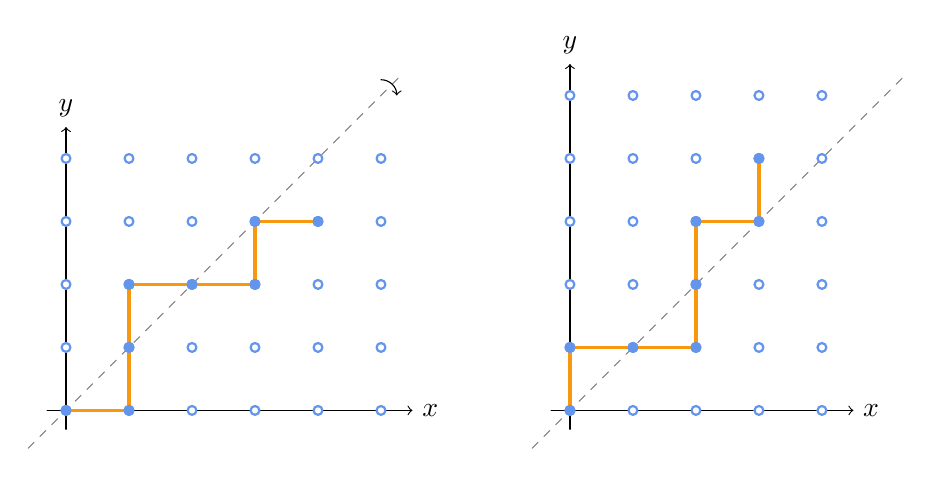
\begin{tikzpicture}[scale=.8,line join=round,line cap=round]
    
    \draw[->] (-0.3,0) -- (5.5,0) node[right] {$x$};
    \draw[->] (0,-0.3) -- (0,4.5) node[above] {$y$};
    \draw[dashed,Gray] (-0.6,-0.6) -- (5.3,5.3);
    
    \foreach \x in {0,1,2,3,4,5} {
      \foreach \y in {0,1,2,3,4} {
        \draw[thick,CornflowerBlue,fill=white] (\x,\y) circle (2pt);
      }
    }

    \coordinate (A1) at (0,0);
    \coordinate (A2) at (1,0);
    \coordinate (A3) at (1,1);
    \coordinate (A4) at (1,2);
    \coordinate (A5) at (2,2);
    \coordinate (A6) at (3,2);
    \coordinate (A7) at (3,3);
    \coordinate (A8) at (4,3);

    \draw[very thick,YellowOrange]
      (A1) -- (A2) -- (A3) -- (A4) -- (A5) -- (A6) -- (A7) -- (A8);
    \foreach \i in {1,2,3,4,5,6,7,8} {
      \draw[thick,CornflowerBlue,fill=CornflowerBlue] (A\i) circle (2pt);
    }

    \begin{scope}[shift={(5,5)}]
      \draw[->] (90:0.25) arc[start angle=90,end angle=0,radius=0.25];
    \end{scope}

    \begin{scope}[shift={(8,0)}]

      \draw[->] (-0.3,0) -- (4.5,0) node[right] {$x$};
      \draw[->] (0,-0.3) -- (0,5.5) node[above] {$y$};
      \draw[dashed,Gray] (-0.6,-0.6) -- (5.3,5.3);
      
      \foreach \x in {0,1,2,3,4} {
        \foreach \y in {0,1,2,3,4,5} {
          \draw[thick,CornflowerBlue,fill=white] (\x,\y) circle (2pt);
        }
      }

      \coordinate (B1) at (0,0);
      \coordinate (B2) at (0,1);
      \coordinate (B3) at (1,1);
      \coordinate (B4) at (2,1);
      \coordinate (B5) at (2,2);
      \coordinate (B6) at (2,3);
      \coordinate (B7) at (3,3);
      \coordinate (B8) at (3,4);

      \draw[very thick,YellowOrange]
        (B1) -- (B2) -- (B3) -- (B4) -- (B5) -- (B6) -- (B7) -- (B8);
        \foreach \i in {1,2,3,4,5,6,7,8} {
          \draw[thick,CornflowerBlue,fill=CornflowerBlue] (B\i) circle (2pt);
        }

    \end{scope}

  \end{tikzpicture}

  \caption[Transposition of lattice walks]{By reflecting a lattice walk through the diagonal we obtain a bijective correspondence between lattice walks to $(m,n)$ and lattice walks to $(n,m)$.}
  \label{figure:lattice-walks}
\end{figure}

\begin{corollary}\label{corollary:transposing-order-preserving-maps}
  There is a bijection
  \begin{equation*}
    \mathrm{Map}_{\leq}(\{1,\ldots,n\},\{0,\ldots,m\}) \cong
    \mathrm{Map}_{\leq}(\{1,\ldots,m\},\{0,\ldots,n\}).
  \end{equation*}
\end{corollary}

\begin{remark}
  While \zcref{corollary:transposing-order-preserving-maps} follows directly from the previous observations, it is worthwhile to construct the bijection $f\mapsto f^\ast$ explicitly.

  Consider an order-preserving map $f:\{1,\ldots,n\}\to\{0,\ldots,m\}$. By the correspondence of \zcref{theorem:stars-and-bars} we obtain $c_i=\#f^{-1}(i)$ such that
  \begin{equation*}
    c_0+\cdots + c_m=n. 
  \end{equation*}
  This determines the subset $\{a_1,\ldots,a_m\}\subseteq\{1,\ldots,m+n\}$ given by $a_1:= c_0$ and $a_{i+1}=a_i+c_i+1$. The complement of this subset is a set $\{b_1,\ldots,b_n\}$

  Thus, $f^\ast : \{1,\ldots,m\}\to\{0,\ldots,n\}$ is the unique order-preserving map such that for any $1\leq i\leq m$ and any $1\leq j\leq n$ we have
  \begin{equation*}
    f(i)\leq j \Leftrightarrow i \leq f^\ast(j).
  \end{equation*}

  The Canadian mathematician Andr\'e Joyal observed that duality between order-preserving maps $\{1,\ldots,n\}\to\{0,\ldots,m\}$ and order-preserving maps $\{1,\ldots,m\}\to\{0,\ldots,n\}$ can be generalized to a duality between planar trees and a combinatorial structure called disks \cite{joyal1997}.
\end{remark}

\begin{theorem}\label{theorem:stars-and-bars-primes}
  Given a set $p_1,\ldots,p_n$ of distinct primes, the set of numbers of the form
  \begin{equation*}
    p_1^{m_1}\cdots p_n^{m_n}
  \end{equation*}
  such that $m_1+\ldots+m_n\leq k$ has exactly $\binom{k+n}{n}$ elements.
\end{theorem}

\begin{proof}
  By the hockey-stick identity (\zcref{exercise:hockey-stick-identity}), we have
  \begin{equation*}
    \sum_{i=0}^k\binom{i+n-1}{n-1}=\binom{k+n}{n}.\qedhere
  \end{equation*}
\end{proof}


\exercises

\begin{starter}
  \exercise In the empty copy of Pascal's triangle at the end of this chapter, shade all the positions of the odd binomial coefficients. It is not necessary to compute them all.
  \exercise Prove that $2^n<n!$ for all $n\geq 4$.
  \exercise Prove that
  \begin{equation*}
    \sum_{k=0}^n \binom{n}{k} = 2^n
  \end{equation*}
  in three different ways: using the binomial theorem, by a direct proof by induction, and by a combinatorial proof.
  \exercise Consider an $n$-element set $X$. We call a bijection $f:X\cong X$ \define{transitive} if $X$ is inhabited and for every two elements $x,y\in X$, there exists a natural number $k$ such that $f^k(x)=y$. How many transitive bijections are there on $X$?
  \exercise Find the first $20$ positive integers that are not divisible by any Fibonacci number other than $1$. % This is https://oeis.org/A147956 
  % \exercise Define the \emph{inclusion-exclusion sequence} $a_n$ by $a_0:=0$, $a_1:=1$, and let $a_{n+1}$ be the largest positive integer so that the number of positive integers $1\leq x < a_{n+1}$ not divisible by any $a_i$ for $2\leq i\leq n$ is $a_n$. Determine the values for $a_n$ for $1\leq n\leq 10$.
\end{starter}

\begin{routine}
  \exercise \label{exercise:estimates-central-binomial-coefficients}Show that the strict inequalities
  \begin{equation*}
    \frac{4^n}{2n+1} < \binom{2n}{n} < 4^n
  \end{equation*}
  hold for all $n\geq 1$.
  \exercise Prove that
  \begin{equation*}
    \sum_{k=0}^n\binom{n}{k}(-1)^k = 0.
  \end{equation*}
  Conclude that
  \begin{equation*}
    \sum_{k=0}^{\lfloor n/2\rfloor}\binom{n}{2k} =\sum_{k=0}^{\lfloor (n-1)/2\rfloor}\binom{n}{2k+1}.
  \end{equation*}
  In this formula, the floor $\lfloor x\rfloor$ of a number $x$ is the largest integer below or equal to $x$.
  \exercise \label{exercise:hockey-stick-identity}\emph{The hockey-stick identity.} Show that
  \begin{equation*}
    \sum_{i=k}^m\binom{i}{k}=\binom{m+1}{k+1}.
  \end{equation*}
  \exercise \emph{The Chu--Vandermonde identity.} Use the binomial theorem at the polynomial $(x+1)^m(x+1)^n$ to show that
  \begin{equation*}
    \sum_{i=0}^k \binom{m}{i}\binom{n}{k-i} = \binom{m+n}{k}.
  \end{equation*}
  \exercise Show that
  \begin{equation*}
    \sum_{k=0}^n \binom{n}{k}^2 = \binom{2n}{n}.
  \end{equation*}
  The binomial coefficient $\binom{2n}{n}$ is also called the \define{central binomial coefficient}.
  \exercise Define a bijection between ordered triples $(a,b,c)$ of positive integers such that $a+b+c=n$ and the set of $2$-element subsets of $\{1,\ldots,n-1\}$, and use this to determine the number of such ordered triples.
  \exercise Consider an arbitrary subset $A$ of the natural numbers, and let the sets $\mathcal{P}_{\mathrm{even}}(A)$ and $\mathcal{P}_{\mathrm{odd}}(A)$ be defined as follows:
  \begin{align*}
    \mathcal{P}_{\mathrm{even}}(A) & :=\big\{S\subseteq A\bigm| \text{$S$ is finite and }{\textstyle \sum_{s\in S}s}\text{ is even}\big\}, \\
    \mathcal{P}_{\mathrm{odd}}(A) & :=\big\{S\subseteq A\bigm| \text{$S$ is finite and }{\textstyle \sum_{s\in S}s}\text{ is odd}\big\}.
  \end{align*}
  Show that there is a bijection bijection $f:\mathcal{P}_{\mathrm{even}}(A)\to\mathcal{P}_{\mathrm{odd}}(A)$ if and only if the set $A$ contains an odd number. Use this bijection to conclude that for $n\geq 1$, there are exactly $2^{n-1}$ subsets $S\subseteq\{1,\ldots,n\}$ whose sum of elements is even.
\end{routine}

\begin{challenge}
  \exercise Show that
  \begin{equation*}
    \sum_{k=0}^n\prod_{i=0}^m (k+i) = (m+1)!\binom{n+m+1}{m+2}.
  \end{equation*}
  \exercise
  \begin{subexenum}
  \item Show that in the $n$\supth{} row of Pascal's triangle all the entries are odd precisely when $n=2^k-1$ for some $k$.
  \item Show that in each row of Pascal's triangle, the number of odd entries is always a power of $2$.
  \end{subexenum}
  \exercise A \define{derangement} is a bijection $f:A\to A$ such that $f(x)\neq x$ for every $x\in A$. We define the \define{derangement number} $!n$ to be the number of derangements on an $n$-element set.
  \begin{subexenum}
  \item Compute $!n$ for $0\leq n\leq 6$.
  \item Show that the derangement numbers satisfy the following recurrence relation:
    \begin{equation*}
      {!(n+2)}=(n+1)({!(n+1)}+{!n}).
    \end{equation*}
  \item Use the principle of inclusion--exclusion to show that
    \begin{equation*}
      !n= {n!}\sum_{k=0}^n \frac{(-1)^k}{k!}.
    \end{equation*}
  \end{subexenum}
\end{challenge}

\cleardoublepage

\thispagestyle{empty}

\begin{figure}[p]
  \makebox[\textwidth][c]{%
  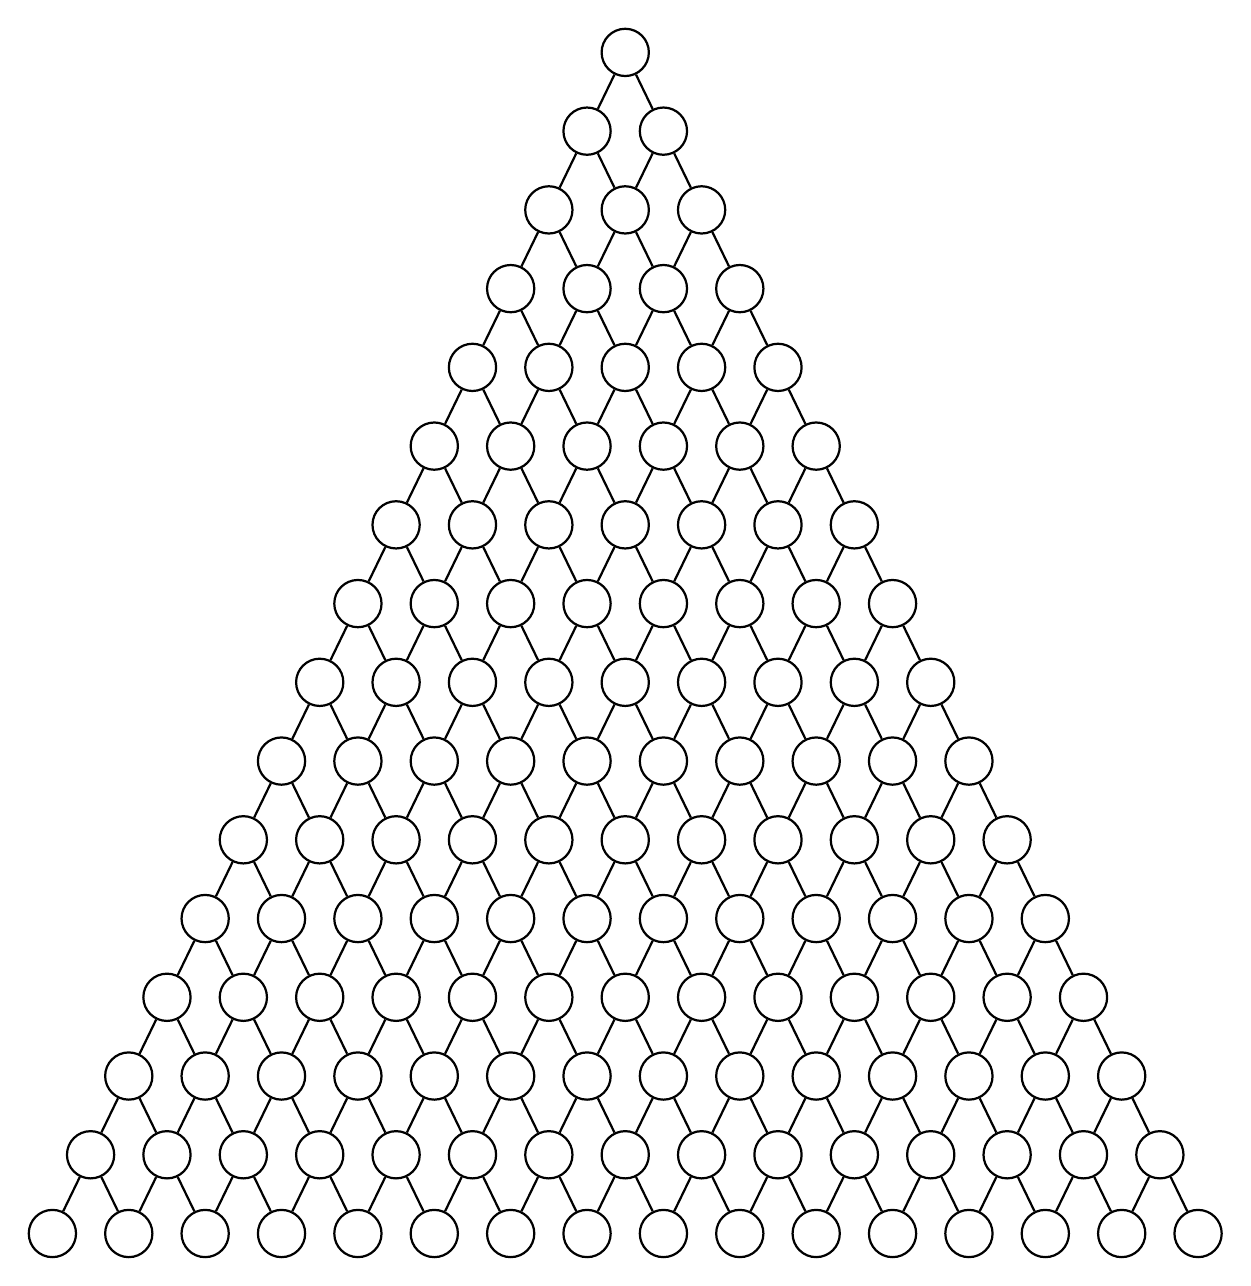
\begin{tikzpicture}[
    x=.97cm,
    every node/.style={
      draw,
      thick,
      circle,
      minimum size=6mm,
      inner sep=0pt,
      align=center
    }]

    \foreach \n in {0,...,15}{
      \foreach \r in {0,...,\n}{
        \node (n\n\r) at (\r-\n/2,-\n) {};
      }
    }
    
    \foreach \n in {0,...,14}{
      \pgfmathtruncatemacro{\nn}{\n+1}
      \foreach \r in {0,...,\n}{
        \pgfmathtruncatemacro{\rp}{\r+1}
        \draw[thick] (n\n\r) -- (n\nn\r) (n\n\r) -- (n\nn\rp);
      }
    }
  \end{tikzpicture}}

  \caption[Parity in Pascal's triangle]
  {Shade all the circles in which the binomial coefficient is odd.}
  \label{figure:parity-pascals-triangle}
\end{figure}

\clearpage

\thispagestyle{empty}

%%% Local Variables:
%%% mode: latex
%%% TeX-master: "number-theory"
%%% TeX-engine: luatex
%%% End:
